\chapter{Theory}
\section{Modelling of light propagation in tissue}
Photon migration through turbid media such as human tissue is usually well described by the radiative transport equation \cite{Durduran2010,Ishimaru1978}. The radiative transport equation, in turn, is well approximated by the diffusion equation for the photon fluence rate when the medium has low absorption but substantial scattering \cite{Ishimaru1978,Rossum1999}. The derivation of the photon diffusion equation from the transport equation can be traced back to nuclear transport theory \cite{Case1967}, and the reader who is interested in the passage from the transport to diffusion equation should consult several useful review articles \cite{Durduran2010,Gibson2005,Venugopal2012}. Herein, we will assume the diffusion approximation is valid for the media we investigate, i.e., human tissues. Thus, for the purposes of this thesis, in a media with low absorption and high scattering, we will assume that the photon fluence rate $\Phi(\mbf{r},t) \ (W/cm^{2})$ obeys the diffusion equation:
%
\begin{equation}
\label{eqn:DEtime}
\nabla\cdot ( D(\mbf{r}) \nabla \Phi(\mbf{r},t)) - v\mu_a(\mbf{r}) \Phi(\mbf{r},t) + S(\mbf{r},t) = \frac{\partial \Phi(\mbf{r},t)}{\partial t}.
\end{equation}
\noindent
Here $\mbf{r}$ represents position in the sample, $t$ is time, $v$ is the speed of light in the medium (i.e., $c/n$ where $c$ is the speed of light in vacuum and $n$ is the index of refraction of the medium), $\mu_a(\mbf{r})\ (\rm{cm^{-1}})$ is the tissue absorption coefficient, $D(\mbf{r})=\frac{v}{3(\mu_a(\bf{r})+\mu_s^{\prime}(\mbf{r}))}$ is the tissue diffusion coefficient wherein $\mu_s'(\mbf{r})~(\rm{cm^{-1}})$ is the tissue reduced scattering coefficient, and $S(\mbf{r},t)\ (\rm{W/cm^{3}})$ is the light source term. In the near-infrared (NIR) wavelength range, typical optical properties of the human breast are $\mu_a\sim 0.05\,\rm{ cm^{-1}}$ and $\mu_s^{\prime}\sim 8\,\rm{ cm^{-1}}$.
\\ \indent
The experiments in this thesis employ frequency-domain (FD) techniques. In the frequency-domain, the light source is typically point-like in space (which we often model with a delta function) and is modulated sinusoidally at an angular frequency $\omega$. In this case, the source and resulting photon fluence rate have DC and AC components. %
\begin{eqnarray}
\label{eqn:DE_ac}
S(\mbf{r},t) & = & [S_{dc} + S_{ac}e^{-i\omega t}]\delta(\mbf{r}-\mbf{r}_s) \ ;\\
\label{I_AC}
\Phi(\mbf{r},t) & = & \Phi(\mbf{r})_{dc} + \Phi(\mbf{r})_{ac}e^{-i\omega t} \ .
\end{eqnarray}
%
\noindent
Here $S_{dc}$ is the DC light source power density (with units $(W/cm^{3})$), $S_{ac}$ is the AC light source power density, and $\mbf{r}_s$ is the source location. Equation (\ref{eqn:DE_ac}) shows that the photon fluence rate also has corresponding AC and DC components. Note, here the equations are expressed using complex notation; in this case, we expect that the AC components for both the source and the fluence rate to be complex. In later chapters, we are mainly concerned with the phase and the amplitude of the AC component of the fluence rate. Substituting for the light source and fluence rate from the two equations above into the diffusion equation, one readily derives the following frequency-domain diffusion equation i.e., equation for the AC component of the fluence rate: 
%
\begin{equation}
\label{eqn:DE}
[-\nabla \cdot D(\mbf{r}) \nabla + v \mu_a(\mbf{r})-i\omega]\Phi({\bf
  r},\omega)=S\delta(\mbf{r}-\mbf{r}_s) \ .
\end{equation}
%
\noindent
For clarity, I have suppressed the AC subscript, and explicitly written the frequency dependence, $\omega$, into the argument of the fluence rate in order to remind the reader of its importance.  Equation~(\ref{eqn:DE}) is the starting point for most of the analyses in this thesis, including the tomographic image reconstruction algorithms. However, before we delve into the tomographic reconstruction, we will solve this equation analytically for some common and simple geometries: homogeneous infinite media, semi-infinite media and slab media.

\subsection{Boundary Conditions}
To find a complete solution to any differential equation, one needs boundary conditions. For infinite medium, the primary requirement is for the photon fluence rate to reduce to zero at infinity. However, in practice, most important situations involve interfaces between diffuse and non-diffuse media, e.g., the air-tissue interface. The boundary condition problem has been discussed in books and review papers \cite{Haskell1994,Aronson1993,Aronson1995,Contini1997, Durduran2010}. Here I provide a review of the key results without detailed derivations.

To accomplish this task, we must return to the transport equation and its key functional quantities. Consider a small volume element centered on the point at $\mbf{r}$. The radiance $L$ ($\rm{W/m^2sr^1}$), is a measure of the light energy per unit area per unit solid angle at $\mbf{r}$ and traveling in the direction $\mbf{s}$. Thus, the isotropic fluence rate, $\Phi(\mbf{r},t)$ in the diffusion equation above is obtained by integrating the radiance over all possible angles/directions; the associated photon flux, $\mbf{j(r)}$, is the vector sum of the radiance emerging from the volume element:
%
\begin{eqnarray}
\Phi(\mbf{r}) &=& \int\int_{4\pi} d\Omega \ L(\mbf{r},\mbf{ s})\ ; \\
\mbf{ j}(\mbf{ r}) &=& \int\int_{4\pi} d\Omega \ L(\mbf{ r},\mbf{ s}) \ \hat{\mbf{ s}} \ .
\end{eqnarray}
\indent
In the diffusion approximation, which is also called the $P_1$ approximation because it only retains spherical harmonics of order zero and one from the transport equation, the radiance only depends on the fluence rate and photon flux. Specifically, at any point, $\mbf{ r}$, the radiance is simply the sum of the isotropic fluence rate at $\mbf{ r}$ plus an additional term involving the dot product of the photon flux at $\mbf{ r}$ and the unit vector along $\mbf{s}$, i.e., 
%
\begin{eqnarray}
L(\mbf{r},\mbf{s}) &=& \frac{1}{4\pi} [ \Phi(\mbf{r}) + 3 \mbf{j}(\mbf{r}) \cdot \hat{\mbf{s}}] \ .
\end{eqnarray}
\ident
Typically, we study diffuse media (like tissue) that are bounded by non-diffuse media (like air). Therefore, we must carefully consider what happens to the radiance at the air-tissue boundary (see Fig.~\ref{fig:boundary}). Let $\mbf{\hat{n}}$ be the outward unit normal on the tissue surface, and let $\mbf{\hat{s}}$ define a direction of the light radiance propagation. In this case, the radiance exiting and entering the tissue at the boundary is determined, respectively, by integrating the radiance over all outward directions ($L(\mbf{s}) (\mbf{\hat{s}} \cdot \mbf{\hat{n}})$) and integrating  the radiance over all inward directions ($L(\mbf{s}) (\mbf{\hat{s}} \cdot - \mbf{\hat{n}})$). Since air is non-scattering medium, the only light radiance that can enter the tissue from the boundary is due to Fresnel (specular) reflections of outgoing light radiance at the boundary. Let $R(\mbf{s})$ be the Fresnel reflection coefficient for unpolarized light at the angle $\theta$ (where $\mbf{\hat{s}}\cdot \mbf{\hat{n}}=\cos\theta$ and $\mbf{\hat{j}}\cdot \mbf{\hat{n}}=j_z\cos\theta$), then
\begin{equation}
\label{eqn:partialflux}
\int\int_{\mbf{\hat{s}} \cdot \mbf{\hat{n}} > 0} R(\mbf{s}) L(\mbf{s}) (\mbf{\hat{s}} \cdot \mbf{\hat{n}}) d\Omega =
\int\int_{\mbf{\hat{s}} \cdot \mbf{\hat{n}} < 0} L(\mbf{s}) (\mbf{\hat{s}} \cdot {- \bf\hat{n}}) d\Omega \ .
\end{equation}
%
\indent
\begin{figure}[t]
\centering
\label{fig:boundary}
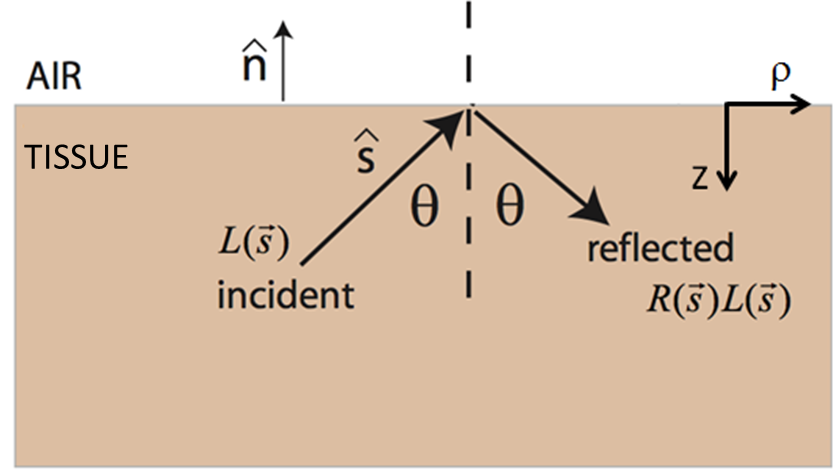
\includegraphics[width=8cm]{./figures/2_Theory/BoundaryReflect.png}
\caption[Diagram of air-tissue boundary]{At the air-tissue boundary, a fraction of the incident radiance $L(\hat{s})$ is Fresnel reflected ($R(\hat{s})$) back into the turbid medium due to index mismatch. This reflected light $R(\hat{s})L(\hat{s})$ accounts for all light diffusing inwards into the medium at the boundary. The boundary condition is derived using this observation. $\hat{n}$ is the unit vector normal to the air-tissue boundary. $z$ increases downward into the tissue and $\rho$ is parallel with the boundary.}
\end{figure}
The solution of this equation leads us to the well-known partial-flux boundary condition \cite{Haskell1994,Aronson1995}, i.e.,
\begin{align}
\Phi + \ell \nabla \Phi\cdot\mbf{\hat{n}} = 0 \label{eqn:BC_DE} \ ; \\ 
\ell = 2D\frac{1+R_{eff}}{1-R_{eff}} \ .
\label{eqn:extrap}
\end{align}
Here $R_{eff}$ is the effective reflection coefficient due to the index of refraction differences at the interface \cite{Orchard1969,Godavarty2002}. The positive parameter, $\ell$ (Equation~\ref{eqn:extrap}), is called the extrapolated boundary length; it corresponds to the distance (along the direction normal to the interface) for which the solution to Equation~\ref{eqn:BC_DE} is zero. (Note, this result is obtained with the Taylor expandsion of the fluence rate around its value at the interface, while keeping only the terms up to first order). Again, the details of this approach have been worked out in \cite{Haskell1994,Aronson1993,Aronson1995,Durduran2010}, and I will not carry out the derivation here. The resulting so-called extrapolated boundary condition is:
\begin{equation}
\Phi(z=-\ell)= 0 \ .
\end{equation}

We will use this extrapolated boundary condition to construct the Green's functions for semi-infinite and slab media. These Green's functions (or some equivalent form), in turn, facilitate solution of the problem when the turbid medium is heterogeneous. Of course, this latter situation is important for imaging inside a breast with cancerous lesions.
%
\subsection{Analytical Solutions}
This section covers three analytical solutions to the photon diffusion equation. We will solve for the fluence rate, $\Phi$, in homogenous turbid media in the infinite, the semi-infinite, and the slab geometries. For the infinite medium, we will derive the Green's function. For the semi-infinite and slab problems we will use the method of images and the extrapolated boundary condition to derive new Green's functions. 

\subsubsection{Infinite Geometry}
The simplest case we consider is the infinite geometry. Starting with the diffusion equation in the frequency domain (Equation~\ref{eqn:DE}), we assume that both the diffusion coefficient and the absorption coefficient of the medium are constant (i.e., the medium is homogeneous). Further, we assume that the point light source sits at the origin of the coordinate system. After dividing both sides by $D$, and defining the constant $k_0^2 = \frac{- v\mua^0 + i\omega}{D}$, (Equation ~\ref{eqn:DE}) can be written in the following Helmholtz-like form:
%
\begin{equation}
\label{eqn:DEhelm}
(\nabla^2+k_0^2)\Phi(\mbf{r},\mbf{r}_s)=-\frac{S}{D}\delta(\mbf{r}-\mbf{r}_s) \ .
\end{equation}
%
\noindent
Note, in this form, the photon fluence rate, $\Phi$, due to a point source is proportional to the Green's function solution (in this case the proportionality constant is $S/D$) for the Helmholtz equation (i.e., for the Helmholtz-like equation above with the unusual wave-vector). This equation for the Green's function with point source at $\mbf{r_s}$ is:
%
\begin{equation}
\label{eqn:Ghelm}
(\nabla^2+k_0^2)G(\mbf{r},\mbf{r}_s)=-\delta(\mbf{r}-\mbf{r}_s) \ .
\end{equation}
%
\noindent
With the boundary condition that the fluence rate goes to zero at infinity we obtain the well-known result:
%
\begin{equation}
\label{eqn:Ginf}
G(\mbf{r},\mbf{r}_s) = \frac{1}{4\pi}\frac{e^{ik_o|\mbf{r}-\mbf{r}_s|}}{|\mbf{r}-\mbf{r}_s|} \ .
\end{equation}
%
This Green's function solution is an overdamped spherical wave that vanishes at infinity. The wave-vector has real and imaginary parts that depend on the absorption coefficient, the reduced scattering coefficient, and the modulation frequency. The photon fluence rate solution is computed by spatial convolution of the Green's function and source distribution (which can originate at only a single point, but need not).
%
\subsubsection{Semi-infinite Geometry}
Now that we have the Green's function solution for infinite media, it is straight-forward to derive related solutions in the semi-infinite geometry. A key assumption from the partial-flux boundary condition facilitates the solution: the fluence rate is zero at the so-called extrapolated boundary (which is typically close to the real air-tissue boundary) \cite{Haskell1994,Aronson1993,Aronson1995}. Thus, if we know the source position, then we can use the method of images to construct our Green's function such that it vanishes at the extrapolated boundary. Recall that the extrapolated zero boundary is located a distance $\ell$ from the air-diffusive media interface ($z=0$) as shown in figure \ref{fig:semiinf}. 

The solution for the semi-infinite geometry can be readily determined using the well-known method of images. If a source exits some distance $\ell + z_s$ away from the extrapolated boundary (i.e., in the turbid medium), then we must place a sink the same distance on the opposite side of the boundary to insure that the net fluence rate at the extrapolated boundary position (i.e., between the real and image sources) is zero (see figure \ref{fig:semiinf}). This method-of-images approach yields the Green's function for the semi-infinite medium. The Green's function with the source and image source is
%
\begin{equation}
\label{semisoln}
G(\rho_s=0,z_s;\rho,z) = \frac{1}{4\pi} \left( \frac{exp[ikr_+]}{r_+} 
- \frac{exp[ikr_-]}{r_-} \right) \ ;
\end{equation}
%
\begin{eqnarray}
\label{ext_both}
r_{+} = & \sqrt{\rho^2+(z-z_{+})^2} \ ; \nonumber \\
r_{-} = & \sqrt{\rho^2+(z-z_{-})^2} \ .
\end{eqnarray}
%
\noindent
Here $z_+=z_s$ is the position of the source and $z_-=-2\ell-z_s$ is the position of our image source. Note, typically the source position due to a light fiber located at the air-tissue interface is set to be at a distance (into the diffuse medium) equal to the reciprocal of the reduced scattering coefficient and measured from the air-tissue interface at $z=0$.  Finally, as was the case for the infinite medium, the photon fluence rate solution is computed by spatial convolution of the Green's function and source distribution (which can originate at a only one point, but need not).
%
\begin{figure}[t]
\centering
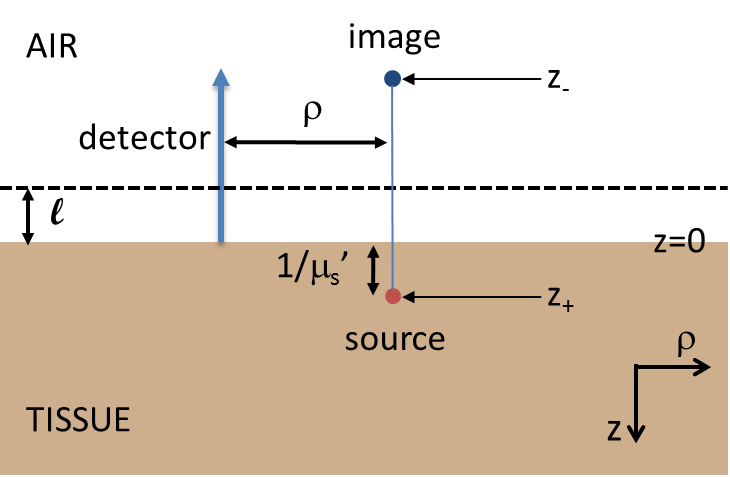
\includegraphics[width=8cm]{./figures/2_Theory/semiinf.png}
\caption[Diagram of the semi-infinite case]{The semi-infinite case where the method of images is used to find the solution of the Green's function. The $z$ direction increases downwards into the medium. $z_+$ is the location of the source, $z_-$ is the location of the image sink, and $z=0$ is the boundary between the tissue and air. The dotted line is where the extrapolated boundary is located a distance $\ell$ away from the boundary. $\rho$ is the distance between the source and detector fibers.}
\label{fig:semiinf}
\end{figure}
%
\subsubsection{Slab Geometry}
The solution for the slab geometry is just a more complicated variant of the solution for the semi-infinite case. We use the method of images again. This time, however, there is a second boundary, and we again make the assumption that $\Phi=0$ some distance $\ell$ away from the air/diffuse-media boundary for the second interface at $z=L$. As in the semi-infinite case, we add an image sink above the top ($z=0$) boundary, but now we also need to add another image sink below the bottom ($z=L$) boundary to the source.
\begin{figure}[h]
\begin{center}
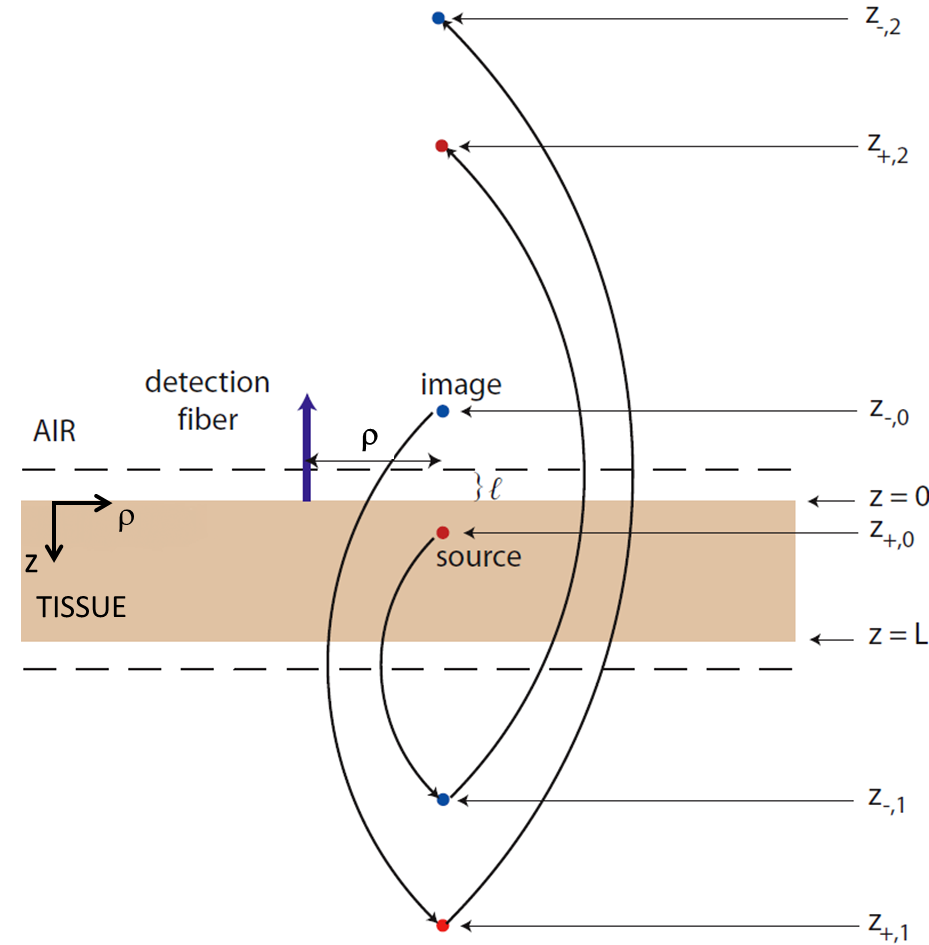
\includegraphics[width=10.5cm]{./figures/2_Theory/slab.png}
\caption[Diagram of the slab case]{The slab case where the method of images is used to find the solution of the Green's function. $z_+,0$ is the location of the source, $z_-,0$ is the location of the image sink, $z_+,1$ is the first source image, $z_-,1$ is the 2nd sink image and so on. $z=0,L$ is location of the boundaries between the tissue and air. The dotted line is where the extrapolated boundaries are located a distance $\ell$ away from the tissue/air boundaries. $\rho$ is the distance between the source and detector fibers. $z$ increases downwards into the slab.}
\label{fig:slab}
\end{center}
\end{figure}

Notably, every additional sink that is added would need its own image source, leading to a recursive procedure of adding sources and sinks. Therefore a pattern in the position of these sources and sinks emerge, and the Green's function for the original source and all the images can be written as an infinite sum:
\begin{equation}
G(\rho_s,z_s;\rho,z) = \frac{1}{4\pi} \sum_{m=-\infty}^{m=\infty} 
\left\{ \frac{exp[ikr_{+,m}]}{r_{+,m}} - \frac{exp[ikr_{-,m}]}{r_{-,m}} \right\} \ ;
\end{equation}
\vspace{-20mm}
\begin{eqnarray}
\label{ext_both}
r_{+,m} = & \sqrt{(\rho-\rho_s)^2+(z-z_{+,m})^2} \ ; \notag \\
r_{-,m} = & \sqrt{(\rho-\rho_s)^2+(z-z_{-,m})^2} \ .
\end{eqnarray}
\noindent
Here $z_{+,m}=2m(L+2\ell)+z_s$, $z_{-,m}=2m(L+2\ell)-2\ell-z_s$, $m=0,\pm 1, \pm 2, ...$, and $L$ is the thickness of the slab. For the semi-infinite geometry, only the $m=0$ term is used. 

Again, typically the source position due to a light fiber located at the air-tissue interface is set to be at a distance (into the diffuse medium) equal to the reciprocal of the reduced scattering coefficient; $z_{+,m}$ is positive as measured from air-tissue interface at $z=0$. Also, the terms in the sum are decreasing in size with distance of the image sources from the primary interface, so one typically does not have to keep too many terms to obtain good agreement between theory and experiment. Finally, as was the case for the infinite medium, the photon fluence rate solution is computed by spatial convolution of the Green's function and source distribution (which can originate at only one point, but need not).
%
\subsection{Multi-spectral Methods}
\subsubsection{Chromophore Absorption}
In tissues and other turbid media, the total absorption, $\mua$, is dependent on the relative concentrations of chromophores within the medium. If the number of chromophores is $N$, and they have spatial concentration distributions $c_i(\mbf{r})$,($i=1..N$), then 

\begin{equation}
\label{eqn:Chromo}
\mu_a(\lambda,\mbf{r}) = \sum_{i=1}^N c_i(\mbf{r}) \varepsilon_i(\lambda) \ .
\end{equation}
Here $\lambda$ is the wavelength of the probing light, and $\varepsilon_i$ is the wavelength-dependent extinction coefficient of chromophore $i$. The $\varepsilon_i$ are typically known from independent spectral measurements. Notice, it is possible to determine the chromophore concentrations, $c_i$, using this linear relationship. That is, the chromophore concentrations can be reconstructed directly from measurements of the absorption coefficient ($\mua$) at multiple wavelengths $\lambda_j$ ($j=1..M$), provided the number of independent equations ($M$) is equal to or greater than the number of unknowns ($N$). 

In breast tissue, the major chromophores are deoxy- (Hb), oxy-hemogloblin (${\rm HbO_2}$), lipid, and water (${\rm H_2O}$) in the near-infrared (NIR) wavelength range. The extinction coefficients for these chromophores are known \cite{Mourant1997,Doornbos1999,Wang2012,Jacques2013}. Furthermore, typical concentration values are known for breast, and this knowledge often helps to provide bounds/constraints on the allowed absorption in tomographic reconstructions. In our reconstructions in Chapter 4 the volume concentrations of water and lipid in the breast is assumed based on values from the literature \cite{Lee1997,White1987,Woodard1986}. 

Various analysis schemes are employed to extract physiological concentration information from the wavelength-dependent data. The traditional method determines an absorption coefficient at each wavelength, and then employs the equation above to extract chromophore concentrations. However, it is also possible to use all data at all wavelengths simultaneously to reconstruct chromophore concentrations. This latter, so-called multi-spectral approach has been shown to stabilize the reconstructions and to improve concentration fidelity \cite{Corlu2003,Srinivasan2005,Li2007}, provided that enough wavelengths are utilized.
%
\subsubsection{Scattering: Spectral Signatures from Mie Theory}
In tissue, the scattering properties are due to a number of factors, especially organelles (e.g., mitochondria, nuclei, cells, cell/tissue interfaces) and their concentration. In practice, the scattering coefficient, $\musp$, has been found to exhibit a power law variation as a function of wavelength in the NIR. Interestingly, this power law follows from a Mie scattering analysis too; the simplest Mie analysis assumes that all of the scattering is due to spherical particles of fixed size, but more complex analyses can add in particle size polydispersity, etc.

Mie scattering is a theory for light scattering from spherical particles based on Maxwell's equations. It is quite general, and it becomes especially important to use when the wavelength of the incident light becomes comparable to the particle size. 

Although Mie theory is old, its application to scattering in tissues in this context is relatively recent \cite{Mourant1997,Bevilacqua2000,Jacques2013}. If we assume a Mie scattering model as described above, then the wavelength dependence of the scattering coefficient,  $\musp$, has a power-law form: 
%
\begin{equation}
\musp(\lambda,\mbf{r}) = a(2\pi\varrho n_m)^b \lambda^{-b}  .
\end{equation}
%
Here $a$ is a constant that is proportional to the scatterer density, $\varrho$ is the radius of the spheres, $n_m$ is the index of refraction of the medium, and $b$ is the scattering power. In biomedical optics, this equation is often further simplified to
%
\begin{equation}
\label{eqn:Mie}
\musp(\lambda,\mbf{r}) = A(\mbf{r}) \lambda^{-b} \ .
\end{equation}
Here $A$ is called the scattering prefactor. A few papers have been published that fit scattering spectra from tissues, and, generally, $b$ is found to vary between 0.5 and 3 \cite{Bevilacqua2000,Jacques2013}. Notice, the spatial distribution of scattering model parameters, $A$ and $b$, can in principle be independently reconstructed from multi-spectral data \cite{Corlu2005}. However, it is quite common for experimenters to assume a fixed value for $b$ and then reconstruct $A$ and hence determine $\musp$. Since the NIR spectral range is not too broad, the scattering wavelength dependence is useful to employ in the reconstructions, which are often not very sensitive to the exact values of $A$ and $b$ in lieu of $\musp$.
%
\section{Reconstruction Methods}
The main rationale for using Diffuse Optical Tomography (DOT) in breast cancer imaging is that tumors have different physiological properties, such as vasculature, metabolic activity, organelle concenrations, and more, compared to surrounding healthy tissue. Furthermore, these differences in physiological properties are reflected as differences in optical properties, such as absorption and scattering coefficients.

Typical DOT instruments send photons into tissue at known points on the tissue surface (sources); output light that has traveled through the breast is then detected at known locations on the breast tissue surface (detectors). Importantly, this work is carried out in geometries that can be modeled reasonably with Green's function-based inverse problem approaches. Within these schemes, we utilize the measured data to solve for unknown $\mua$ and $\musp$ values in each volume element of the 3-dimensional image-space for the medium. Common reconstruction methods require two basic steps: 1) solving the forward problem and 2) solving the inverse problem (see Fig.~\ref{fig:forwardinverse}).

The forward problem, in essence, involves solving the diffusion equation for the fluence rate at known locations (e.g., within the medium or at the detector positions). The forward solution is readily determined, provided we are given specific values of $\mua$ and $\musp$ in each volume element within the sample, as well as information about input source locations and the tissue boundaries.

Solving the inverse problem is conceptually and technically more difficult than the forward problem. It involves determining new values of $\mua$ and $\musp$ from a comparison of the fluence rate at the boundary to the forward problem solution. Generally, as experimenters, we have knowledge about the diffuse light that we send into the medium and about the light that we measure after its emergence from the medium. The task of the inverse problem is to find unique solutions for the optical properties inside the medium, given this information.
%
\begin{figure}[t]
\centering
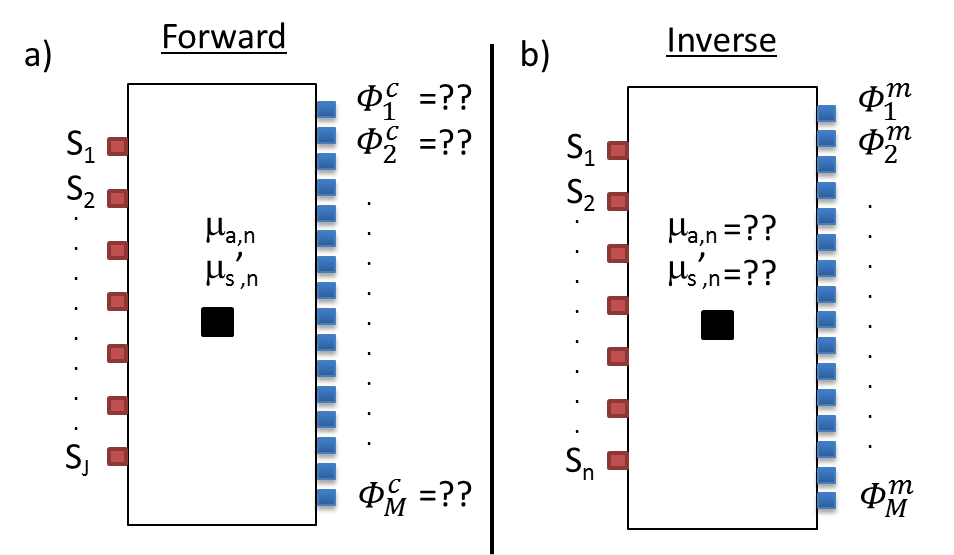
\includegraphics[width=10.5cm]{./figures/2_Theory/forwardinverse.png}
\caption[Forward and inverse problem diagrams]{a) Forward problem diagram (model) for slab geometry. The forward problem calculates the fluence $\Phi_{model}$ at detector locations, given values for the source ($S$) locations as well as $\mua$ and $\musp$ at $N$ voxel locations inside the turbid medium. b) Inverse problem diagram (experimental). From the measured value for the fluence at the boundaries $\Phi_{data}$, and the calculated fluence rate from the forward problem, the values for $\mua$, $\musp$ are updated/calculated.}
\label{fig:forwardinverse}
\end{figure}

For the forward problem, general theoretical approaches can be divided into three groups: Analytical methods, Numerical methods, and Monte-Carlo (MC) methods. These schemes range, respectively, from least to most computationally demanding. The analytical method is the fastest and easiest scheme (if we can figure out the analytic solution); given the source distribution, sample geometry, and optical properties, all that is required is a Green's function to generate the fluence rate within the medium (and on its boundaries). In principle, these analytical or semi-analytical approaches are well suited to use with very large data sets. However, the analytical approaches have limitations. These limitations come, in part, from “true” experimental geometries that differ from ideal cases and other experimental limitations such as small heterogeneities in the medium. Numerical methods, though more computationally intensive, are a bit more versatile. For example, by using numerical schemes, the number of assumptions about geometry are reduced, and it is possible to utilize well-worn techniques such as the Finite Element Method (FEM) and Finite Difference Method (FDM). The Monte-Carlo approach is a stochastic method which employs random step or Markov-chain models to account for transport of photons through the tissue; each of these photon trajectories is traced through the medium, with probability of absorption and scattering events included, until the photon exits or is absorbed. Though probably the most accurate method, this procedure employs a large number of photons ($>10^8$) and thus very computationally and time intensive. Of the methods described above, we will primarily investigate the first two groups.

The inverse problem is inherently more difficult than the forward problem; it involves the inversion of matrices (or similar/related mathematical operations). Such inversions are necessary to solve/update $\mua$ and $\musp$ from the measured and calculated fluence rates.  Standard inversions of the resulting sets of linear equations are non-trivial. For example, they can involve generating a pseudoinverse matrix (e.g., using singular value decomposition (SVD)). These operations are fast but are susceptible to large deviations due to the ill-conditioned matrices and noise, among other factors. A different approach to derive a solution is iterative and nonlinear (to varying degrees). In the nonlinear case, an iterative approach is utilized wherein the measured fluence is compared to the forward model (e.g., FEM model) solution of the diffusion equation using a cost function $\mbf{\Psi}$ (see Section \ref{sec:inverse}). The key iteration step chooses a direction in the solution-space and calculates (e.g., using either the Conjugate-Gradient (CG) method or the Gauss-Newton (GN) method) new optical property parameters; then the forward problem is solved again (with the new optical properties) and the iteration steps are repeated until a pre-set convergence criteria is reached. The nonlinear methods, while more accurate and flexible, are computationally very expensive and time consuming, especially when the data sets and the number of volume elements are large.

In the following sections we describe two inverse problem approaches using analytic (Section~\ref{sec:Analytic}) and algebraic (Section~\ref{sec:Algebraic}) linear schemes. Further, these reconstructions are used to analyze the experimental data described in Chapter 3. We will also discuss a nonlinear reconstruction method which is used for the experimental data in Chapter 4.
%
\subsection{Linear Reconstruction Methods}
\label{sec:linearrecon}
\subsubsection{Linearized Integral Equations}
\label{sec:rytov}
Here we derive linear solutions to the diffusion equation (\ref{eqn:DE}) in turbid media with heterogeneities. To simplify our problem, we divide the absorption and scattering (i.e., light diffusion coefficient) parameter into two parts: homogeneous background components and spatially heterogeneous (i.e., perturbative) components:
%
\begin{align}
\mua(\mbf{r}) &= \mua^0+\delta\mua(\mbf{r}) \ ; \\
D(\mbf{r}) &= D^0+\delta D(\mbf{r}) \ .
\end{align}

We use/substitute this perturbation expansion of the optical properties into the diffusion equation (Equation~\ref{eqn:DE}) in the presence of a single \textbf{point source} at $\mbf{r}_s$ (and we replace the fluence rate, $\Phi$, with the corresponding Green's function, $G$). Note, again, formally the fluence rate in this situation, $\Phi(\mbf{r}_s,\mbf{r})$, is proportional to the Green's function, $G(\mbf{r}_s,\mbf{r})$. Rearranging this resulting equation as described, we obtain:
%
\begin{equation}
\label{eqn:DEdiff}
\left[ - D^0 \nabla^2 + v\mu_a^0 - i\omega \right]G(\mbf{r}_s,\mbf{r})= \delta(\mbf{r}-\mbf{r}_s) - \Big[v\delta\mua(\mbf{r})-\nabla \cdot \delta D(\mbf{r})\nabla\Big] G(\mbf{r}_s,\mbf{r}) \ .
\end{equation}

The LHS of this equation is essentially the homogeneous diffusion equation with average/background values of absorption and diffusion. The spatially heterogeneous perturbations introduce important additional terms on the RHS of the equation. These terms account for how the fluence rate propagation is modified by the heterogeneous perturbations. We can manipulate this equation to derive an expression for the Green's function, $G(\mbf{r}_s,\mbf{r}_d)$, for a particular source-detector pair where $\mbf{r}_d$ is the detector position. The Green's function satisifes the Dyson equation:
\begin{equation}
\label{eqn:Dyson}
G(\mbf{r}_s,\mbf{r}_d) = G_0(\mbf{r}_s,\mbf{r}_d) - \int_V G_0(\mbf{r},\mbf{r}_d) [\delta\mu_a(\mbf{r}) - \nabla \cdot \delta D(\mbf{r}) \nabla] G(\mbf{r}_s,\mbf{r}) \ d^3 r \ .
\end{equation}
\noindent
Here the integral is taken over $V$, the full volume of our medium (i.e., the slab), and $G_0(\mbf{r}_s,\mbf{r}_d)$ is the analytic Green's function solution for the homogenous medium, i.e., homogenous slab, in this case.

This equation is intrinsically nonlinear, since $G(\mbf{r}_s,\mbf{r})$ depends on the optical properties too. Linearization involves the recursive substitution of the Green's function $G(\mbf{r}_s,\mbf{r})$ in the integrand, with Equation~\ref{eqn:Dyson}. The higher order terms are then neglected, leading to a linearized equation, where we have now excluded $G(\mbf{r}_s,\mbf{r})$ from the RHS. In addition, to simplify the notation, we let $\alpha(\mbf{r})=[v\delta\mu_a(\mbf{r}) - \nabla \cdot \delta D(\mbf{r}) \nabla]$. The lowest order linear solution, as might be expected from any Born expansion, is: 
\begin{align}
\label{eqn:LinDyson}
G(\mbf{r}_s,\mbf{r}_d) = G_0(\mbf{r}_s,\mbf{r}_d) - \int_V G_0(\mbf{r},\mbf{r}_d) \alpha(\mbf{r}) \
G_0(\mbf{r}_s,\mbf{r}) \ d^3 r \ .
\end{align}
\noindent
If, instead of the Born approximation the first Rytov approximation~\cite{Schotland1997} is adopted, Equation~(\ref{eqn:LinDyson}) yields: 
\begin{equation}
\label{eqn:linearDE}
G(\mbf{r}_{\rm d}, \mbf{r}_{\rm s}) = G_0(\mbf{r}_{\rm d}, \mbf{r}_{\rm s})
\exp\left[ -\int_V \frac{ G_0(\mbf{r}_{\rm d}, \mbf{r}) \alpha(\mbf{r})
G_0(\mbf{r}, \mbf{r}_{\rm s})\,d^3r}{G_0(\mbf{r}_{\rm d}, \mbf{r}_{\rm s})} \right] .
\end{equation}

Now let us connect this result to the data we might measure in an experiment. In practice, two independent measurements of the transmitted intensity are made. (Note, this intensity is derived from and is proportional to the diffuse light fluence rate at the output plane.) One measurement is made on a homogeneous (reference) media, and the another measurement is made on the medium with heterogeneities (i.e., the medium we want to understand). We denote these measurements by $I_0(\mbf{r}_{\rm d}, \mbf{r}_{\rm s})$ and $I(\mbf{r}_{\rm d}, \mbf{r}_{\rm s})$, respectively, where $\mbf{r}_{\rm d}$ and $\mbf{r}_{\rm s}$ are vectors specifying the positions of the detector and the source. Note, in my experimental work in Chapters 3 and 4, these quantities, $I_0$ and $I$, are ultimately derived from measured CCD counts in particular CCD pixels with specific integration times; the number of CCD counts in each pixel is linearly proportional to the corresponding photon fluence rate from the detected region. These measurements are readily connected to Green's function (which is also proportional to the fluence rate) and thus related to the optical properties of the sample medium through the relations:
\begin{align}
\label{eqn:Intensity1}
I(\mbf{r}_d, \mbf{r}_s) &= C_d(\mbf{r}_d)C_s(\mbf{r}_s)G(\mbf{r}_d,\mbf{r}_s) \ ; \\
\label{eqn:Intensity2}
I_0(\mbf{r}_d, \mbf{r}_s) &= C_d(\mbf{r}_d)C_s(\mbf{r}_s)G_0(\mbf{r}_d,\mbf{r}_s) \ .
\end{align}
\noindent

As noted above, $G(\mbf{r}_d,\mbf{r}_s)$ is the Green's function solution that is proportional to the fluence rate we should measure with our CCD. The quantities $C_d(\mbf{r}_d)$ and $C_s(\mbf{r}_s)$ are unknown coupling coefficients on the detectors and sources respectively. The coupling coefficients are cancelled out (in principle) when we normalize the true sample data by the reference measurement for the reconstructions (i.e., when we compute $I/I_0$).

We divide both sides of Equation~\ref{eqn:linearDE} by $G_0$, and take the natural log of both sides of the resulting equation. Finally we multiply both sides by $-G_0$ and obtain:
\begin{align}
-G_0(\mbf{r}_{\rm d}, \mbf{r}_{\rm s}) \ln\bigg[\frac{G(\mbf{r}_{\rm d}, \mbf{r}_{\rm s})}{G_0(\mbf{r}_{\rm d}, \mbf{r}_{\rm s})}\bigg] &= \int_V G_0(\mbf{r}_{\rm d}, \mbf{r}) \alpha(\mbf{r}) G_0(\mbf{r}, \mbf{r}_{\rm s})\,d^3r \ ; \\
\phi(\mbf{r}_d,\mbf{r}_s) &= \int_V G_0(\mbf{r}_{\rm d}, \mbf{r}) \alpha(\mbf{r}) G_0(\mbf{r}, \mbf{r}_{\rm s})\,d^3r \ .
\label{eqn:linearphi}
\end{align}
Here we define the so-called Rytov data function, $\phi(\mbf{r}_d,\mbf{r}_s)$ as
\begin{equation}
\label{eqn:datafunction}
\phi(\mbf{r}_d,\mbf{r}_s) =-G_0(\mbf{r}_{\rm d}, \mbf{r}_{\rm s}) \ln\bigg[\frac{I(\mbf{r}_{\rm d}, \mbf{r}_{\rm s})}{I_0(\mbf{r}_{\rm d}, \mbf{r}_{\rm s})}\bigg] \ .
\end{equation}
\noindent
Note, that the data function $\phi(\mbf{r}_d,\mbf{r}_s)$ is proportional to the measured fluence rate $\Phi(\mbf{r}_d,\mbf{r}_s)$. The right-hand side of the equation above contains the measured data function, and the left-hand side is an integral transform of the contrast within the sample. This formulation of the linearized DOT inverse problem is standard~\cite{Schotland1997}. 

\subsubsection{Analytical Inverse Reconstruction}
\label{sec:Analytic}
The analytical inverse reconstruction method that describe here and use in Chapter 3 was pioneered by my collaborators \cite{Markel2001,Markel2002,Markel2002a,Markel2003,Markel2003a,Markel2004,Konecky2008a}. Its application in the slab geometry has been reported in Refs.~\cite{Wang2005,Konecky2008a,Ban2013}. In this method, the inverse problem is simplified by taking advantage of symmetries which reduce the complexity of the Green's function while also enabling simplified data inversions through the use of the Fourier transform. To achieve this goal, one first decomposes the Green's function into plane waves so that it has the following form:
\begin{equation}
\label{eqn:Gplanes}                                               
G(\mbf{r},\mbf{r}^{\prime}) = \frac{1}{(2\pi)^3}\int d^3k \ g(k) \ e^{i\mbf{k} \cdot (\mbf{r}-\mbf{r}^{\prime})} \ .
\end{equation}
Here $g(k)$ gives the amplitude and phase for each plane wave. For complex boundaries, it is impossible to solve for $g(k)$. However, for some simple symmetric geometries (i.e., semi-infinite, slab, cylindrical, spherical), formulas for the Fourier components can be derived \cite{Markel2002a}.
\begin{figure}
\label{fig:slabcoord}
\centering{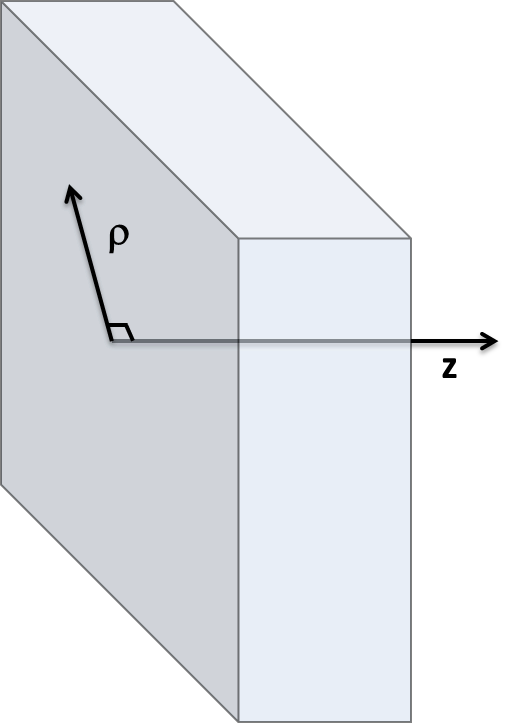
\includegraphics[width=5.5cm]{./figures/2_Theory/slabcoord.png}}
\caption[Slab geometry diagram]{Coordinates in the slab geometry. The positive z direction points into the slab while $\rho$ is parallel to the surface.}
\end{figure}

Our experiments in Chapters 3 and 4 are carried out in the slab geometry. Therefore, we will study the specifics of the slab geometry. In the slab, we define $\mbf{r} = (\mbf{\rho},z)$ where $z$ is depth in the medium and $\mbf{\rho}$ is parallel to the surfaces (see Fig.~\ref{fig:slabcoord}). In the Fourier space, $\mbf{k}=(\mbf{q},k_z)$. The form of the Helmholtz equation is thus modified: 
\begin{equation}
\label{eqn:slabhelm}
(\nabla^2_{{\bm \rho}} + \frac{\partial^2}{\partial z^2} + k_0^2)G(\mbf{r},\mbf{r}^{\prime}) = \frac{-1}{D_0} \delta (\mbf{r}-\mbf{r}^{\prime}) \ .
\end{equation}
Since no translational symmetry exists in the $z$ direction, we expand the Greens function in plane waves along ${\bm \rho}$. Then
\begin{equation}
\label{eqn:G_slab}
G(\mbf{r},\mbf{r'}) = \frac{1}{(2\pi)^2} \int d^2q \ g(q,z,z') e^{i\mbf{q} \cdot ({\bm \rho}-{\bm \rho}^{\prime})} \ .
\end{equation}
\label{eqn:g_1d}
Substitution of Equation~\ref{eqn:G_slab} into Equation~\ref{eqn:slabhelm} gives a one-dimensional differential equation for each value of $\mbf{q}$.
\begin{equation}
\left(\frac{\partial^2}{\partial z^2} - (q^2-k_0^2) \right) g(q,z,z') = \frac{-1}{D} \delta (z-z') \ .
\end{equation}
Although I will not write out the derivation here (see reference \cite{Konecky2008,Konecky2008a}), please note that g(q,z,z') can be solved for in the slab geometry and has the form:
\begin{equation}
\label{eqn:g_slab}
g(q;z,z') = \frac{\ell}{D} \frac{{\rm sinh}[Q(L-|z-z'|)]+Q\ell {\rm cosh}[Q(L-|z-z'|)]}{{\rm sinh}(QL)+2Q\ell {\rm cosh}(QL)+(Q\ell)^2{\rm sinh}(QL)}
\end{equation}
where $Q = q^2 -k_0^2$, $L$ is the slab thickness, and $\ell$ is the extrapolated boundary distance.

\subsubsection{Fourier Inversion Equations}
We next derive the inversion equations. We begin by substituting the plane wave Green's function (Equation~\ref{eqn:G_slab}) into the linearized forward equation we must solve (i.e., Equation~\ref{eqn:linearphi}). This substitution yields the following equation for the data function:
%
\begin{eqnarray}
\label{eqn:linearphiG}
\phi(\mbf{r}_s,\mbf{r}_d) = & \frac{1}{(2\pi)^4} \int d^2q_s \int d^2q_d \int d^3r \ g(q_d,z,z_d) {\rm exp}[i\mbf{q}_d \cdot ({\bm \rho} - {\bm \rho}_d)] \ ; \nonumber \\
 & \times \alpha(\mbf{r}) \ g(q_s,z_s,z) {\rm exp}[i\mbf{q}_s \cdot ({\bm \rho}_s - {\bm \rho})] \ .
\end{eqnarray}
%
For discrete source-detector pairs, the Fourier transform and the substitution of $\mbf{q} = \mbf{q}_s + \mbf{q}_d$, and $\mbf{p}=-\mbf{q}_s$, gives us a set of separate integral equations for each value of $q$:
%
\begin{equation}
\label{eqn:1Dfourier}
\tilde{\phi}(\mbf{q}_s, \mbf{q}_d) = \int_{z_s}^{z_d} \ \left[
\kappa_A(\mbf{q}_s,\mbf{q}_d;z)\ c \ \delta \tilde{\mu}_a(\mbf{q}_s+\mbf{q}_d) +
\kappa_D(\mbf{q}_s,\mbf{q}_d;z) \ \delta \tilde{D}(\mbf{q}_s+\mbf{q}_d) \right] dz
\end{equation}
%
where
\begin{align}
\label{kappaA}
\kappa_A(\mbf{q},\mbf{p};z) & = g(-\mbf{p};z_s,z) g(\mbf{q}+\mbf{p};z,z_d) \ ; \\
\label{kappaD}
\kappa_D(\mbf{q},\mbf{p};z) & = \frac{\partial g(-\mbf{p};z_s,z)}{\partial z}\frac{\partial g(\mbf{q}+\mbf{p};z,z_d)}{\partial z}+\mbf{p} \cdot (\mbf{q}+\mbf{p}) \ g(-\mbf{p};z_s,z) g(\mbf{q}+\mbf{p};z,z_d) \ .
\end{align}
%
Each integral in Equation~(\ref{eqn:1Dfourier}) can be inverted independently, thereby reducing computation time. From these results, we obtain inverse equations for $\mua$ and $D$ (and thus $\musp$).

Specifically:  1) we compute the Fourier transform of Equation~(\ref{eqn:linearphiG}) to obtain Equation~(\ref{eqn:1Dfourier}); 2) then we solve for $\delta \mua(\mbf{q},z)$ and $\delta D(\mbf{q},z)$ using singular value decomposition; 3) finally, the inverse Fourier transform for a given value of $z$ is computed with the equations below.
\begin{equation}
\delta \mu_a(\mbf{r}) = \frac{1}{(2\pi)^2} \int d^2q {\rm exp}(-i \mbf{q} \cdot {\bm \rho}) \sum_{\mbf{r},\mbf{p}} \kappa_A^*(\mbf{q},\mbf{r};z) \ [\kappa\kappa^*]^{-1}(\mbf{q},\mbf{r},\mbf{p}) \tilde{\phi}(\mbf{q},\mbf{p}) \ .
\end{equation}
\begin{equation}
\delta D(\mbf{r}) = \frac{1}{(2\pi)^2} \int d^2q {\rm exp}(-i \mbf{q} \cdot {\bm \rho}) \sum_{\mbf{r},\mbf{p}} \kappa_D^*(\mbf{q},\mbf{r};z) \ [\kappa\kappa^*]^{-1}(\mbf{q},\mbf{r},\mbf{p}) \tilde{\phi}(\mbf{q},\mbf{p}) \ .
\end{equation}
Here $\kappa_A^* [\kappa\kappa^*]^{-1}$ is the SVD pseudoinverse.

As an aside, note that the computational complexity of the analytical reconstruction is $O(N_q N_p^3)$, where $N_q$ is the number of discrete values of the vector $\mbf{q}$, and $N_p$ is the number of discrete values of $\mbf{p}$ in Equation~\ref{eqn:1Dfourier}. In the numerical implementation of the analytical method in Chapter 3, we have closely followed reference~\cite{Konecky2008a} and used a total of $49\times3249\simeq1.6\times10^5$ independent Fourier-space data points. Using these parameters, the necessary computations require $7\times 10^{9}$ floating point operations. On a single-core Intel Core 2 Duo processor with a peak performance of 19 GFlops, this calculation translates to 7 minutes of computation time.

\subsubsection{Algebraic Method}
\label{sec:Algebraic}
\label{subsec:alg_rec}
In general, variants of the algebraic image reconstruction are among the most popular methods per linear inversion techniques that have been applied to DOT \cite{Kak1987,OLeary1995,Ntziachristos2000,Intes2002}. These reconstructions are obtained by discretization of the volume integral in Equation~(\ref{eqn:linearphi}) and subsequent computation of the pseudo-inverse of the obtained system of linearized equations~\cite{Gonatas1995}.  This method does not require large windows (i.e., it does not need the large field-of-views which are required by symmetry in the analytic inversions), and it can be used with any type of data restriction. For the case of the analytical reconstruction method, on the other hand, for data restriction, it must be assumed that the data function $\phi=0$ (see Equation~(\ref{eqn:linearphi}) at these data points (i.e., $\Phi / \Phi_0=1$ at these restricted data points). On the other hand, the algebraic method requires explicit volume discretization in terms of voxels, while the analytical method allows one to reconstruct the target $z$ plane without much additional effort and is not dependent on volume discretization.

For the purpose of obtaining algebraic reconstructions we divide the slab into cubic voxels. In the discretization we approximate the integral in Equation~(\ref{eqn:linearphi}) with a Riemann sum, resulting in a system of algebraic equations $Ax=\phi$ where $A_{mn}$ is the $M\times N$ weight matrix, where $M$ is the number of distinct source-detector pairs, $N$ is the number of voxels, $x_n = \delta\alpha(\mbf{r}_n) / \alpha_0$ is the vector of dimensionless contrast $(n=1,\dots,N)$, and $\phi_m$ is the $m$-th data point $(m=1,\dots,M)$.  The equations are cast in dimensionless form by defining a dimensionless Green's functions according to $\tilde{G}_0(\mbf{r}, \mbf{r}^\prime) = D_0 h G_0(\mbf{r}, \mbf{r}^\prime)$, where $D_0$ is the diffusion coefficient in the background solution. Then we have:
%
\begin{align}
\label{eq6}
A_{mn} &= (k_{\rm d} h)^2 \tilde{G}_0(\mbf{r}_{{\rm d}m}, \mbf{r}_n) \tilde{G}_0(\mbf{r}_n, \mbf{r}_{{\rm s}m}) \ ; \\
\phi_m &= -\tilde{G}_0(\mbf{r}_{{\rm d}m}, \mbf{r}_{{\rm s}m}) \ln\left[\frac{I(\mbf{r}_{{\rm d}m}, \mbf{r}_{{\rm s}m})} {I_0(\mbf{r}_{{\rm d}m}, \mbf{r}_{{\rm s}m})}\right] .
\end{align}
%
\noindent
Here $k_d=\sqrt{\alpha_0/D_0}$, $\mbf{r}_n$ is the position of the center of the $n$-th voxel, and $\mbf{r}_{{\rm d}m}$, $\mbf{r}_{{\rm s}m}$ are the detector and source positions of the $m$-th data point used in the reconstruction.

The pseudoinverse solution to the above system of equations is defined as the unique solution to the system $(A^*A + \lambda^2 I)x = A^*\phi$, where $\lambda$ is the regularization parameter and $I$ is the identity matrix. In the experiments in Chapter 3, the number of measurements $M$ is much larger than the number of voxels $N$ (e.g., $M\sim 10^7$ and $N\sim 10^4$). Correspondingly, the most time consuming part of finding the pseudoinverse (at least, with the numerical approach we used) is the computation of the matrix product $A^*A$. In the most challenging case considered, we have used $M=2\times 10^7$ and $N=2\times 10^4$, which requires $8\times 10^{15}$ floating point operations. 

On an 8-core Xeon workstation with the peak performance of 56 GFlops, this calculation translates into 40 hours of computation time. However, this time-consuming procedure need only be repeated once for a given source-detector arrangement and given optical properties of the background medium; this situation is the case for my experiment in Chapter 3. Importantly, the resultant matrix, $A^*A$, once computed, can be stored on a hard drive and re-used for image reconstruction with each new data set obtained, e.g., for various positions of the chest wall phantom.  Furthermore, computation of the projection, that is, of the $N$-component vector $A^*\phi$, involves only one matrix-vector multiplication, and its computational cost is insignificant. In our case, the matrix $A^*A$ is small enough to be diagonalized; its eigenvectors and eigenvalues can be also stored on a hard drive for future use. In the reconstructions of Chapter 3, however, we solved the equation $(A^*A+\lambda^2I)x=A^*\phi$ directly by the conjugate-gradient descent method \cite{Hestenes1952}.

\subsection{Nonlinear Reconstruction Methods}
For the approaches described thus far, the tomography problem was linearized. Ultimately, however, it is desirable to employ nonlinear methods to find the solution, because in general the relationship between the measurements made and the unknown optical parameters is nonlinear. Among the advantages of the nonlinear reconstruction methods is that one typically has no restrictions on the experimental geometry; further, no linear assumptions are made to solve the diffusion equation, i.e., as we did in Section~\ref{sec:rytov}. While these conditions usually result in the problem being computationally intensive and time consuming, this drawback is typically compensated with parallelization of the problem. The nonlinear method we employ in this thesis is a model-based reconstruction technique. A forward model of light propagation generates an expected fluence rate, and then we seek to iteratively minimize the differences between our measurement and our model (forward) data by updating the parameters in the forward model. The forward model (diffusion equation) is solved using the finite element method (FEM).
%
\subsubsection{Finite Element Method}
\label{sec:FEM}
The FEM programs I employ are already standardized functions in most inversion software. Nevertheless, here I will quickly describe the basic premise of FEM for DOT, and I refer the interested reader to the literature for a more complete treatment \cite{Arridge1993,Paulsen1995}. To solve the forward problem with FEM, we first define a diffusion equation operator $\mathcal{L} =-\nabla \cdot D(\lambda)\nabla+\mua(\lambda)+i\omega/v$ such that: 
\begin{equation}
\label{eqn:DE_FEM}
\mathcal{L}\Phi(\mbf{r})=q_0(\mbf{r}) \ .
\end{equation}
Here $q_0(\mbf{r})$ is a our source term (note, it doesn't have to be a point source). The boundary condition used here is the Robin-type (partial flux) boundary condition: 
%
\begin{equation}
\Phi(r_b)+ \frac{D(z_b)}{\alpha}\mbf{\hat{n}}\cdot\nabla\Phi(r_b)=0 \ .
\end{equation}
Here $r_b$ is a point on the measurement boundary and $\alpha$ is a refractive index mismatch term \cite{Arridge2000}. Assuming that our detected signal is the normal component of the photon flux $\phi_m = \mbf{\hat{n}}\cdot[-D(r_b)\nabla\Phi(r_b)]$, the equation in the case of the Robin boundary condition simplifies to
\begin{equation}
\phi_m(r_b)=\alpha\Phi(r_b) \ .
\end{equation}

The volume $\Omega$ we are interested in imaging (in our case the slab) is discretized into $V$ vertex nodes. If $ u_i(\mbf{r})$ is a basis function from a V-dimensional subspace, then the approximate piecewise continuous polynomial FEM solution to $\Phi(\mbf{r})$ is 
\begin{align}
\Phi^h(\mbf{r})= \sum_i^V \Phi_i u_i(\mbf{r}) \ .
\end{align}
\noindent
The linear or higher order basis functions are defined over triangle (2D), tetrahedral (3D), or square grid elements (3D, used in TOAST++ \cite{Schweiger2014}).

To find the appropriate basis vectors $u_i(\mbf{r})$, we minimize the residual defined as:
\begin{align}
\label{eqn:FEM_R}
\mathcal{L}\Phi(\mbf{r}) - q_0(\mbf{r})
&= R, \\
&= \sum_i^V R_i u_i(\mbf{r}) \ ,
\end{align}
%
by requiring that $R$ be orthogonal to $u_i$ (for $i=1...V$) which in Equation~\ref{eqn:FEM_R} gives
\begin{equation}
\label{eqn:FEM}
(\mbf{K}(D) + \mbf{C}(\mua) + i\omega\mbf{B} + \alpha\mbf{A})\mbf{\Phi}= \mbf{Q} \ ;
\end{equation}
\begin{align}
K_{ij} &= \int_\omega D(r)\nabla u_i(\mbf{r})\cdot\nabla u_j(\mbf{r}) d\Omega \ ; \\
C_{ij} &= \int_\omega \mua(r) u_i(\mbf{r})u_j(\mbf{r}) d\Omega \ ; \\
B_{ij} &= \frac{1}{v}\int_\omega u_i(\mbf{r})u_j(\mbf{r}) d\Omega \ ; \\
A_{ij} &= \int_{\dell\omega} u_i(\mbf{r})u_j(\mbf{r}) d(\dell\Omega) \ ;
\end{align}
\begin{equation}
q_{0,i} = \int_{\omega} \mua(r) u_i(\mbf{r})q_0(\mbf{r}) d\dell\Omega \ .
\end{equation}
Here $\mbf{\Phi}$ is the FEM basis expansion coefficient vectors for $\Phi(\mbf{r})$. These equations are the FEM discretization of the diffusion equation. Note that $\mbf{K},\mbf{C},\mbf{B},$ and $\mbf{A}$ are matrices of size $V\times V$. Equation~(\ref{eqn:FEM}) can can be inverted to give us our forward solver using Cholesky factorization (CW only), LU Decomposition, or iterative solvers like the Conjugate-Gradient method and GMRES.

\subsubsection{The Inverse Problem}
\label{sec:inverse}
The central problem to image reconstruction lies in finding a solution vector $\mbf{\hat{x}}$ that best fits the measurement data where
\begin{equation}
\mathbf{x}=[\mua_{,1},\cdots,\mu_{,V},\musp_{,1}, \cdots, \musp_{,V}]^T \ .
\end{equation}
The elements of $\mathbf{x}$ are $\mua$ and $\musp$ (at a single wavelength) for every vertex of the volume that we want to reconstruct. A straightforward way to utilize multi-spectral data is to reconstruct $\mbf{x}$ for each wavelength, and then convert $\mua$ and $\musp$ to $C_i$ (where $i$ indexes the chromophore) and $A$ using the relationship given by Equation~(\ref{eqn:Chromo}) and (\ref{eqn:Mie}). (Note, the exponent $b$ can also be a free parameter if desired but is often fixed). It has been learned that multi-spectral methods stabilize various inverse problems \cite{Corlu2005,Corlu2003}, so the preferred method (when the data quality is good for many wavelengths) is to reconstruct for $C_i$ and $A$ utilizing all the data simultaneously in the inversion. Then $\mbf{x}$ is instead
\begin{equation}
\mathbf{x}=[C_{1,1},\cdots,C_{1,V}, \cdots, C_{K,1},\cdots, C_{K,V}, A_1, \cdots, A_V]^T
\end{equation}
\noindent
where the number of elements in $\mbf{x}$ is $N=[(K+1)\times V]$.

Finding the solution vector $\mbf{\hat{x}}$ can be approached as an optimization problem \cite{Arridge1998,Schweiger2005} wherein the solution $\mathbf{\hat{x}}$ is found by minimizing an objective function
%
\begin{equation}
\mbf{\hat{x}} = \arg \min_{\mbf{x}} \Psi(\mbf{x}) \ ,
\end{equation}
\noindent
where above we search for some parameter \mbf{x} that returns the minimum of $\Psi(x)$. Here $\Psi$ is defined
%
\begin{equation}
\label{eqn:Psi}
\Psi = \frac{1}{2}\sum_{l=1}^L\sum_{s=1}^S\sum_{d=1}^{D_s}\Big[\Phi^c(\mbf{x})-\Phi^m\Big]^2 \ .
\end{equation}
\noindent
The summations are over all source-detector pairs and wavelengths in the data sets, where $L$ is the number of wavelengths, $S$ is the number of source positions, and $D_s$ is the number of detector positions for a given source. The total number of measurements is $\ M=L\times(\sum_{s=1}^S D_s)\ $. $\Phi^c(\mbf{x})$ is the fluence rate calculated by our forward FEM (Section~\ref{sec:FEM}) and $\Phi$ is our measured fluence rate for a given source-detector pair, and thus the term to minimize is $[\Phi^c(\mbf{x})-\Phi]^2$.
%
\begin{figure}[h]
\centering
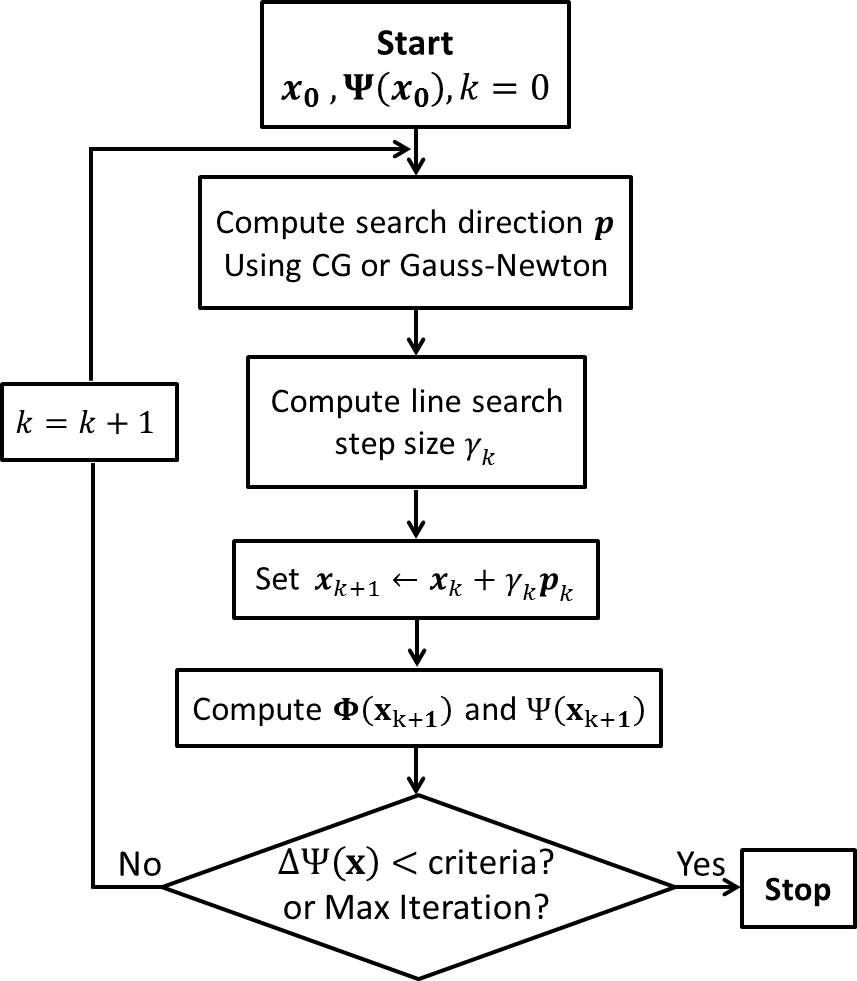
\includegraphics[width=9cm]{./figures/2_Theory/reconflow.png}
\caption{Reconstruction flowchart.}
\label{fig:reconflow}
\end{figure}
%
Fig.~\ref{fig:reconflow} is the flowchart for the image reconstruction algorithms. We start with an initial guess $\mbf{x_0}$ for the parameters, and then calculate the $\Psi$ function by solving the forward problem for $\mbf{\Phi^c(x)}$ and using the measured data $\mbf{\Phi^m}$. The parameter vector $\mbf{x_0}$ is updated by adding a scaled vector $\Delta \mbf{x} = \gamma_k\mbf{p_k}$. Then $\Psi$ is recalculated with the updated parameter vector and checked again to determine if the stopping criteria, which is set by the user to test how close the model fluence rate is to the data, is satisfied. If the criteria, or some maximum iteration number, is not met, then $x$ is updated again, and the loop is continued.

$\Delta\mbf{x}$ depends on the step size $\gamma$ and the step direction $\mbf{p}$. $\gamma$ is determined by a line search along $\mbf{p_k}$ that sufficiently minimizes $\Psi$:
\begin{equation}
\min_{\gamma}\mbf{\Psi(x}_k+\gamma\mbf{p_k}).
\end{equation}
The Taylor's expansion of our updated objective function $\mbf{\Psi(x}_k+\gamma\mbf{p}_k})$ is:
\begin{equation}
\label{eqn:PsiTaylor}
\mbf{\Psi(x}_k+\gamma\mbf{p}_k}) = \mbf{\Psi(x})_k+\gamma\mbf{p}_k^T\nabla\mbf{\Psi(x}_k) + \frac{1}{2}\gamma^2 \mbf{p}_k^T\nabla^2\mbf{\Psi(x})_k\mbf{p}_k + \cdots
\end{equation}
%
The search direction $\mbf{p}_k$ can be derived using either the first order derivative (Conjugate Gradient) or the second order derivative (Gauss-Newton). We will briefly discuss these methods in the following sections.
%
\subsubsection{Conjugate Gradient Method}
The Conjugate-Gradient technique is a commonly implemented method in DOT reconstruction algorithms. For a detailed derivation of the Conjugate Gradient (CG) method, I refer the reader to \cite{Arridge1998,Shewchuk1994}. Very briefly, to use the CG method, $\nabla\mbf{\Psi}$ from the 2nd term of Equation~(\ref{eqn:PsiTaylor}) is needed. It is
\begin{align}
\nabla\mbf{\Psi(x)} &= \mbf{J(x)^T F(x)} \label{eqn:dPsi} \ ; \\
f_i(\mbf{x}) & =\Phi^c_i(\mbf{x})-\Phi^m_i \ ; \\
\mbf{F(x)} &= \Big[f_1(\mbf{x}),f_2(\mbf{x}),\cdots,f_{M}(\mbf{x})\Big]^T \ .
\end{align}
where the Jacobian is
\begin{equation}
J=
\begin{bmatrix}
    \frac{\partial f_1(\mbf{x})}{\partial x_1} & \frac{\partial f_1(\mbf{x})}{\partial x_2} & \cdots & \frac{\partial f_1(\mbf{x})}{\partial x_N} \\
    \frac{\partial f_2(\mbf{x})}{\partial x_1} & \frac{\partial f_2(\mbf{x})}{\partial x_2} & \dots  & \frac{\partial f_2(\mbf{x})}{\partial x_N} \\
    \vdots & \vdots & \ddots & \vdots \\
   \frac{\partial f_M(\mbf{x})}{\partial x_1} & \frac{\partial f_M(\mbf{x})}{\partial x_2} & \dots  & \frac{\partial f_M(\mbf{x})}{\partial x_N}
\end{bmatrix} \ .
\end{equation}

For real experimental data in Chapter 4, the Jacobians are arranged as shown in Fig.~\ref{fig:jacobill}. The Jacobian is typically calculated for known $\mua$ and $\musp$. The image reconstruction software that we use (Toast++) readily provides the gradients for the standard DOT optical coefficients, i.e., 
\begin{equation}
f'^{(\mu_a)} = \frac{\partial \Phi}{\partial \mu_a}, \quad f'^{(\mu_s)} = \frac{\partial \Phi}{\partial \mu_s} \ .
\end{equation}
For multi-spectral data, we want the Jacobian to be written in terms of the chromophore concentration and the scattering factor and power A, b. The required gradients with respect to these parameters can be obtained by applying the chain rule:
\begin{eqnarray}
f'^{(c_i)} &=& \sum_{j=1}^L f'^{(\mu_a)}(\lambda_j) \frac{\partial \mu_a(\lambda_j)}{\partial c_i} = \sum_{j=1}^L f'^{(\mu_a)}(\lambda_j) \varepsilon_i(\lambda_j) \ ; \\
f'^{(A)} &=& \sum_{j=1}^L f'^{(\mu_s)}(\lambda_j) \frac{\partial \mu_s(\lambda_j)}{\partial A} = \sum_{j=1}^L f'^{(\mu_s)}(\lambda_j) \lambda_j^{-b} \ ; \\
f'^{(b)} &=& \sum_{j=1}^L f'^{(\mu_s)}(\lambda_j) \frac{\partial \mu_s(\lambda_j)}{\partial b} = \sum_{j=1}^L f'^{(\mu_s)}(\lambda_j) A \lambda_j^{-b} \ln{\lambda_j} \ .
\end{eqnarray}
%
Now we are able to use the Conjugate Gradient algorithm:
\begin{enumerate}[noitemsep]
\item Initialize: $k=0$
\vspace{-17mm}
\begin{align}
\mbf{r}_0 &=-\nabla\mbf{\Psi(x}_0) \ ; \\
\mbf{p}_0 &= \mbf{r}_0 \ .
\end{align}
\item Find step size (find $\gamma$):
\vspace{-10mm}
\begin{equation}
\min_{\gamma}\mbf{\Psi(x}_k+\gamma_k\mbf{p_k}) \ .
\end{equation}
\item Update parameters:
\vspace{-10mm}
\begin{equation}
\mbf{x}_{k+1} = \mbf{x}_{k} + \gamma_k \mbf{p}_{k} \ .
\end{equation}
\item Check \Big[$\mbf{\Psi(x}_{k+1})<$ criteria?\Big]: ~~~~~~\textbf{Yes:} Stop ~~~~~~\textbf{No:} Continue
\vspace{4mm}
\item Update direction vector:
\vspace{-17mm}
\begin{align}
\mbf{r}_{k+1} &=-\nabla\mbf{\Psi(r}_{k+1}) \ ; \\
\beta_{k+1} &= \frac{\mbf{r}^T_{k+1}(\mbf{r}_{k+1}-\mbf{r}_{k})}{\mbf{r}^T_{k}\mbf{r}_{k}} \ ; \\
\mbf{p}_{k+1} &= \mbf{r}_{k+1} + \beta_{k+1}\mbf{p}_{k} .
\end{align}
\item \vspace{-5mm} $k=k+1$. Move to Step 2.
\end{enumerate}
\begin{figure}[h]
\centering
\label{fig:jacobill}
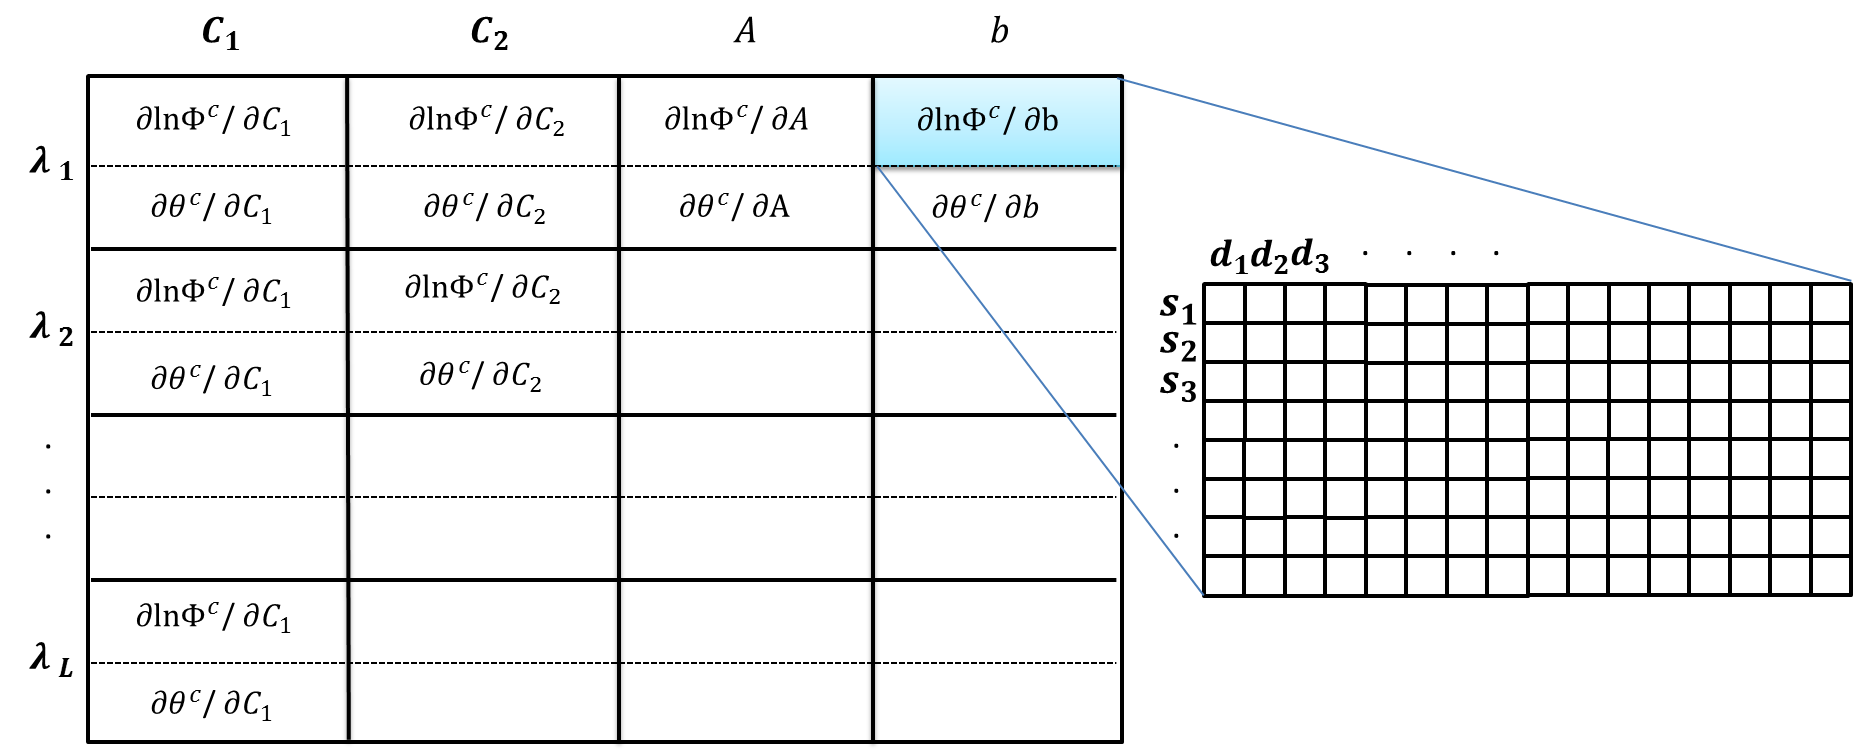
\includegraphics[width=14.5cm]{./figures/2_Theory/jacobschem.png}
\caption[Illustration of the Jacobian matrix for Gen3 imager datasets]{Illustration of the Jacobian matrix for datasets collected in Chapter 4. Row blocks are organized by wavelengths; they are further divided into amplitude and phase. Column blocks are organized by the chromophores ($C$), and A,b. The amplitude and phase data blocks (light blue) consist of data for every source-detector pair: the rows indexes the sources $s$ and the columns indexes the detectors $d$ for each source. }
\end{figure}
%
\subsubsection{Gauss-Newton Method}
The Gauss-Newton method is an iterative method that uses an approximation of second order derivatives in the cost function. Consider Equation~(\ref{eqn:PsiTaylor}) with $\gamma=1$. Let us assume that $\mbf{\Psi(x}_k+\gamma\mbf{p}_k})$ is twice differentiable. Beginning with Equation~(\ref{eqn:PsiTaylor}) and differentiating both sides with respect to $\mbf{p}_k$ we have:
%
\begin{equation}
\nabla\mbf{\Psi(x}_k+\gamma\mbf{p}_k}) = \nabla\mbf{\Psi(x}_k) + \nabla^2\mbf{\Psi(x})_k\mbf{p}_k \ .
\end{equation}
%
$\mbf{\Psi(x}_k+\gamma\mbf{p}_k})$ is minimized when $\nabla\mbf{\Psi(x}_k+\gamma\mbf{p}_k})=0$. The above equation then becomes:
%
\begin{equation}
\nabla^2\mbf{\Psi(x})_k\mbf{p}^{GN}_k = -\nabla\mbf{\Psi(x}_k) \ ,
\end{equation}
\noindent
where $\mbf{p}^{GN}_k$ is a vector that points in the Newton direction. We know $\Big[\nabla\mbf{\Psi(x}_k) = \mbf{2J(x}_k)^T \mbf{F(x}_k)\Big]$ from Equation~(\ref{eqn:dPsi}). $\nabla^2\mbf{\Psi(x})$ is
%
\begin{equation}
\nabla^2\mbf{\Psi(x}_k)=\sum_{m=1}^M\nabla^2(\mbf{\Psi(x}_k)^2)=\sum_{m=1}^M\mbf{H^m(x}_k) \ ,
\end{equation}
where $\mbf{H}^m(\mbf{x}_k)$ is the Hessian. Written out explicitly:
\begin{equation}
\nabla^2\mbf{\Psi(x}_k)= 2\mbf{J(x}_k)^T\mbf{J(x}_k)+\sum_{m=1}^M\sum_{i=1}^N\sum_{j=1}^N f_i(\mbf{x})\frac{\partial f_m(\mbf{x})}{\partial x_i \partial x_j} \ .
\end{equation}
\noindent
The second term is much smaller than the first term, and in the Gauss-Newton method an approximation is made wherein the second term is ignored such that:
%
\begin{equation}
\nabla^2\mbf{\Psi(x}_k)=2\mbf{J(x}_k)^T\mbf{J(x}_k) \ .
\end{equation}
%
Thus the main equation in the Gauss-Newton method is:
%
\begin{equation}
\label{eqn:GN}
2\mbf{J(x}_k)^T\mbf{J(x})_k\mbf{p}_k^N = -\mbf{2J(x}_k)^T \mbf{F(x}_k) \ .
\end{equation}

With this method to ascertain the Gauss-Newton direction $\mbf{p}_k^N$, this relation can be used repeatedly in an iterative manner. A line search method can also be added into the algorithm where the minimum is searched for along $\mbf{p}_k^N$. The Gauss-Newton algorithm is as follows:
\begin{enumerate}[noitemsep]
\item Initialize: k = 0
\item Evaluate:
\vspace{-17mm}
\begin{align}
\nabla\mbf{\Psi(x}_k) &= \mbf{2J(x}_k)^T \mbf{F(x}_k) \ ;\\
\nabla^2\mbf{\Psi(x}_k)&=2\mbf{J(x}_k)^T\mbf{J(x})_k \ .
\end{align}
\item Solve for $\mbf{p}_k^N$ in 
\vspace{-17mm}
\begin{align}
2\mbf{J(x}_k)^T\mbf{J(x})_k\mbf{p}_k^N &= -\mbf{2J(x}_k)^T \mbf{F(x}_k) \\
&{\rm(using~GMRES,~CG,~etc.)} \ . \notag
\end{align}
\item Compute $\gamma_k$ (line search) \ .
\item Update parameter:
\vspace{-10mm}
\begin{equation}
\mbf{x}_{k+1} = \mbf{x}_{k} + \gamma_i \mbf{p}_{k} \ .
\end{equation}
\item Check \Big[$\mbf{\Psi(x}_k)<$ criteria?\Big]: ~~~~~~\textbf{Yes:} Stop ~~~~~~\textbf{No:} Continue
\vspace{4mm}
\item Update $k=k+1$, go to Step 2.
\end{align}
\subsubsection{Levenberg-Marquardt Method}
The Levenberg-Marquardt Method is another technique commonly used in DOT reconstruction packages (e.g., TOAST++, NIRFAST) that I will very briefly summarize. The Levenberg-Marquardt Method is a variation on the Gauss-Newton method wherein a term is added to the Hessian in Equation~\ref{eqn:GN}
\begin{align}
2[\mbf{J(x}_k)^T\mbf{J(x})_k+\lambda I]\mbf{p}_k &= -\mbf{2J(x}_k)^T \mbf{F(x}_k)\ ; \label{eqn:LM-2}\\
\mbf{p}_k &= -2[\mbf{J(x}_k)^T\mbf{J(x})_k]^{-1}\mbf{2J(x}_k)^T \mbf{F(x}_k) \label{eqn:LM-2}\ .
\end{align}
$\lambda$ is called the damping parameter. This additional term has two main effects. The first effect is to increase the the number on the diagonals and therefore suppress the 2nd derivatives. A large $\lambda$ will result in the left hand side of the equation being more like the identity matrix, resulting in the steps becoming more like the steepest descent method. One common technique is to start with a large $\lambda$ and then decrease its value at each iteration (i.e., by half every iteration); this procedure causes a gradual switch from the gradient descent method to Gauss-Newton over each step of the reconstruction. The second effect that this additional term introduces is to limit the step size. Since they are inversely related with the search direction vector $\mbf{p}_k$ (Equation \ref{eqn:LM-2}), higher damping terms have the effect of decreasing the step size. This decrease in step size prevents large changes in the iteration at early steps which is useful when there could be instabilities due to errors in the initial guess. Overall these two functions have an effect of stabilizing the reconstruction in the early iterations.

\subsubsection{Regularization}
\label{sec:reg}
The image reconstruction problems we discussed above are generally ill-posed  and often under-determined (i.e., the number of independent measurements are less than the number of unknowns). Among the characteristics of ill-posed problems is that small changes in detected signals can induce large changes in the reconstructed optical properties This situation implies that the reconstructions have non-uniqueness problems and will require additional constraints to help achieve convergence. In practice the solution space is constrained or \textit{regularized} to utilize \textit{apriori} information. Generally, any scientist working on ill-posed image reconstruction (or ill-posed inverse problems) will utilize some type of regularization technique to optimize their images. In the medical imaging field, regularization is common.

For our nonlinear methods, regularization is typically introduced as a term in the objective function as shown below:
\begin{equation}
\Psi = \frac{1}{2}\sum_{l=1}^L\sum_{s=1}^S\sum_{d=1}^{D_s}\Big[\Phi^c(\mbf{x})-\Phi\Big]^2 + \Lambda R(\mbf{x})\ .
\end{equation}
\noindent
Here $\Lambda$ is the scaling factor, and $R(\mbf{x})$ is called the regularization functional. As in Equation~\ref{eqn:Psi}, $L$ is the total number of wavelengths, $S$ is the total number of sources, and $D_s$ is the number of detectors for a particular source $s$. The additional term can be thought of as a penalty on the cost function based on the regularization functional. A few examples are: $R=||\mbf{x-x_0}||^2_2$,  $R=||\nabla\mbf{x}||_1$, and $R=-\nabla\cdot(\nabla \mbf{x}/|\nabla\mbf{x}|)$; in these cases, the reconstruction is effectively penalized for large optical property excursions within the image based on, respectively, its difference, its gradient, or a function of its change in gradient. The relative importance of these  penalties is adjusted through the scaling factor $\Lambda$, which can be modified with each iteration as well. These kinds of regularization terms are useful when spatial information about the optical properties of the medium are known, or when some information about the optical property variations are expected. The more information one has in advance, the more that can be included in the cost function.

Throughout this thesis, I have explored the utility of various regularization schemes, and I have tried to identify the best ones for our problem. These tasks are non-trivial and have only just begun. In our reconstructions in Chapter 4, we found that the Total Variation (TV) method, which is an edge-preserving regularization, can work well. TV was applied to preserve contrast and to preserve transverse size of targets in our DOT reconstructions, but it also had the cost of increasing certain classes of artifacts. The particular form we used is $\Lambda\sqrt{|\nabla\mbf{x}|^2+\beta^2}$, which is actually an approximation of the TV method. Here $\beta>0$ is a small parameter added to deal with the non-differentiability of the absolute value $|\nabla\mbf{x}|$ when $\nabla\mbf{x}=0$. It is worth noting that it is also possible to employ different regularization multiplicative scaling terms for different optical parameters. For example, in our reconstructions in Chapter 4, we found that using a separate regularization factor for absorption and for scattering improved the spatial fidelity of the target reconstructions (see Section~\ref{sec:2Dsim} in Chapter 4).
